\documentclass[aspectratio=169]{beamer}\usepackage[utf8]{inputenc}
\usepackage[english]{babel}
\usepackage{color}
\usepackage{amsmath,mathtools}
\usepackage{mathptmx}
\usepackage[11pt]{moresize}
\setbeamertemplate{navigation symbols}{}
\setbeamersize{text margin left=5mm,text margin right=5mm}
\usepackage{wrapfig}
\usepackage{bbm}
\usepackage{xcolor}
\usepackage{tabularx}
\usepackage{bm}
\usepackage{lmodern}
\usepackage{algorithm2e}


\newcommand{\R}{\mathbb{R}}
\newcommand{\E}{\mathbb{E}}
\newcommand{\N}{\mathbb{N}}
\newcommand{\Z}{\mathbb{Z}}
\newcommand{\V}{\mathbb{V}}
\newcommand{\Q}{\mathbb{Q}}
\newcommand{\K}{\mathbb{K}}
\newcommand{\C}{\mathbb{C}}
\newcommand{\T}{\mathbb{T}}
\newcommand{\I}{\mathbb{I}}

\setbeamertemplate{caption}[numbered]

\title{On the Uncertainty of Wind Power Generation}
% \subtitle{ Waleed Alhaddad \ Raul Tempone \ Ahmad kebaier }

\author{ Waleed Alhaddad\textsuperscript{\textasteriskcentered} \qquad Ahmed Kebaier\textsuperscript{\ddag} \qquad Ra\'ul  Tempone\textsuperscript{\textasteriskcentered}\textsuperscript{\textdagger} \\  \vskip 0.2in
\textsuperscript{\textasteriskcentered}CEMSE Division, KAUST , Saudi Arabia
 \\ \textsuperscript{\ddag}Université Paris 13, Sorbonne Paris Cité, LAGA, CNRS (UMR 7539) , France  \\ \textsuperscript{\textdagger}Alexander von Humboldt Professor, RWTH Aachen University,  Germany}

\begin{document}
\setbeamercolor{background canvas}{bg=blue!10}


\begin{frame}
\titlepage
\end{frame}

\begin{frame}[label=guide]\frametitle{ Introduction }
Integration of renewable resources into the urban power grid is a challenge due to uncertainties in power production. We focus on wind power. Reliable wind power production forecasting is crucial to:
\begin{itemize}
\item \textbf{Optimization of the price of electricity} for different users such as electric utilities, Transmission system operator (TSOs), Electricity Service providers (ESPs), Independent power producers (IPPs), and energy traders.
\item \textbf{Allocation of energy reserves} such as water levels in dams or oil and gas reserves.
\item \textbf{Operation scheduling} of conventional power plants.
\item \textbf{Maintenance planning} such as that of power plants components and transmission lines.
\end{itemize}

\end{frame}

\begin{frame}\frametitle{Status quo }
  Wind power forecasts can be generally categorized as follows:
  \begin{itemize}
    \item physical models
    \item statistical methods
    \item artificial intelligence methods
    \item spatial correlation methods
    \item persistence models
    \item other hybrid approaches
  \end{itemize}
 The output of such methods is usually a \textbf{deterministic forecast}. Occasionally probabilistic forecasts are produced through uncertainty propagation in the data, parameters or through forecast ensembles. However, little has been done in terms of producing \textbf{data driven probabilistic forecasts} based on the real-world performance of forecasting models.
\end{frame}

\begin{frame}\frametitle{Data}
This is a year long data set from Uruguay based on \textbf{10 minute observation interval of one thousand 72-hour paths} (2018).
\begin{figure}
  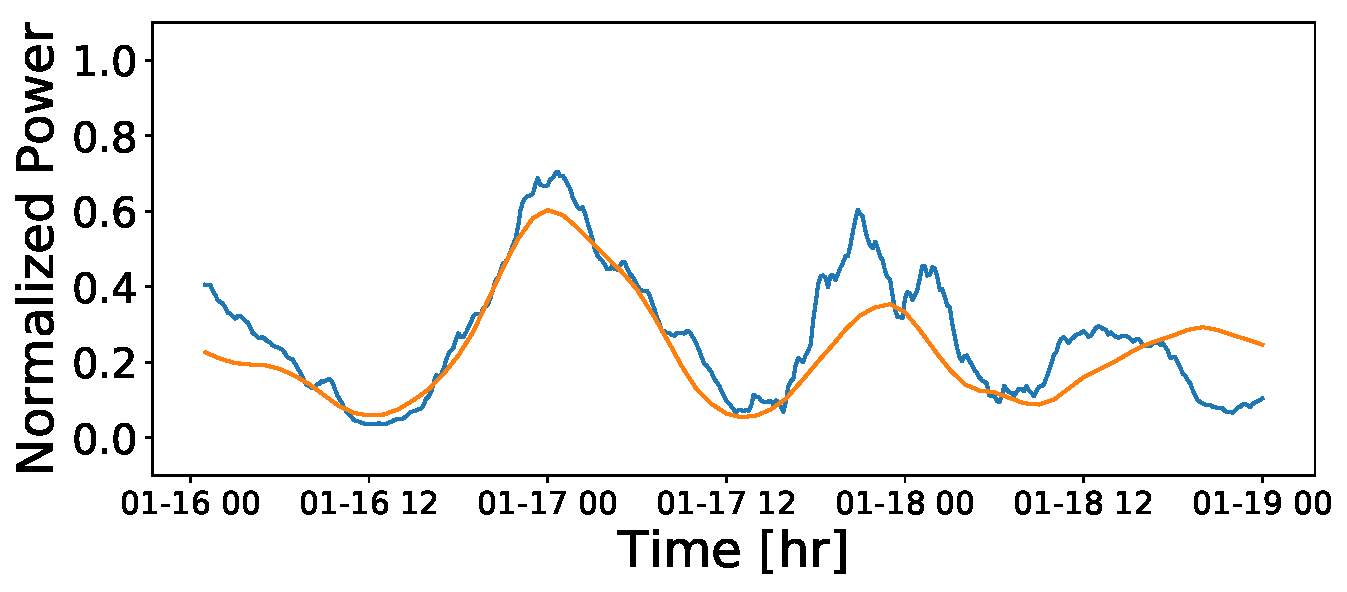
\includegraphics[width=70mm,scale=1]{plots/data_1516064400.pdf}
  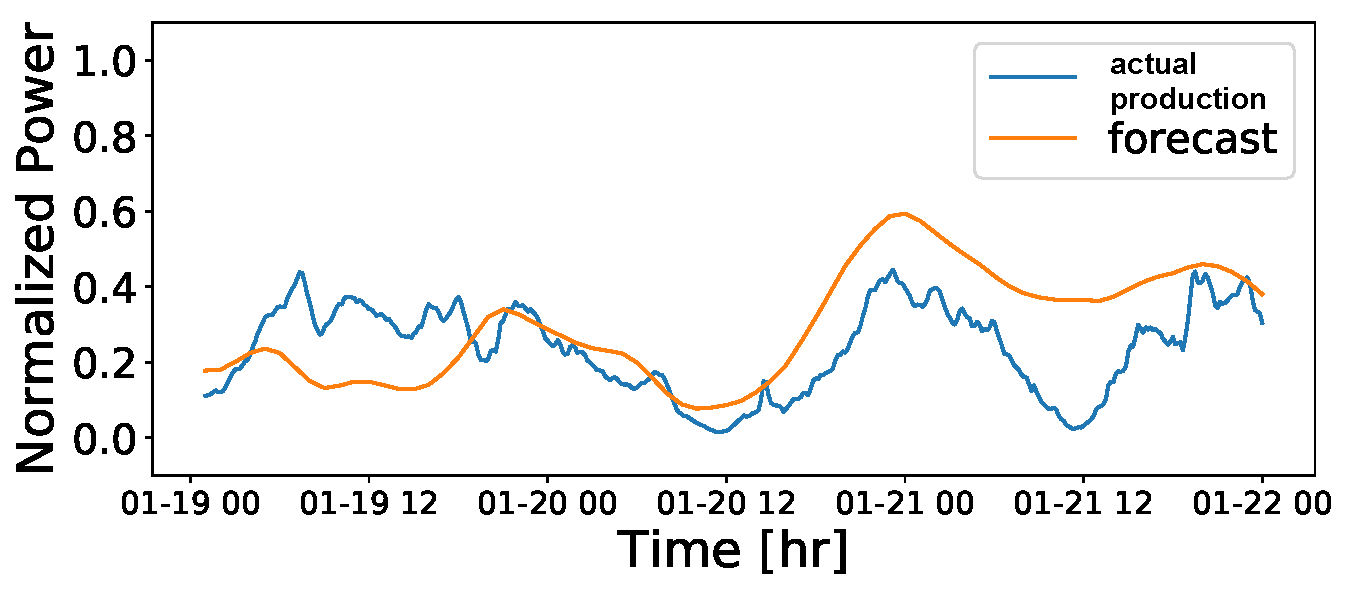
\includegraphics[width=70mm,scale=1]{plots/data_1516323600.pdf}\\
  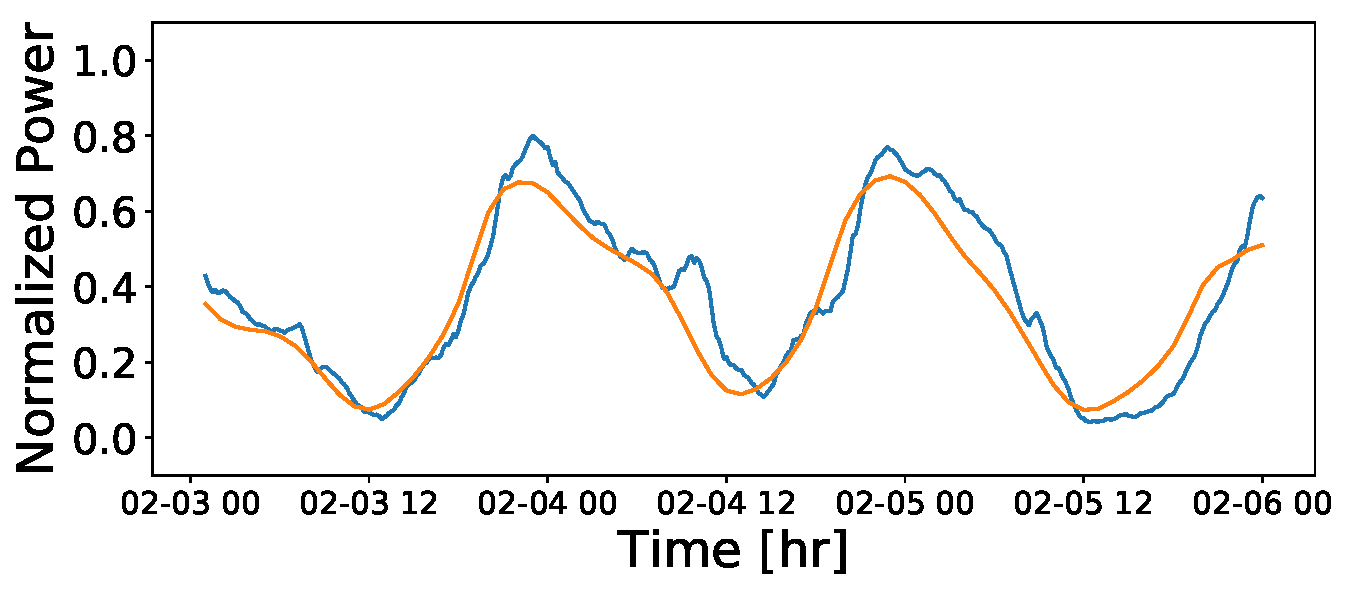
\includegraphics[width=70mm,scale=1]{plots/data_1517619600.pdf}
  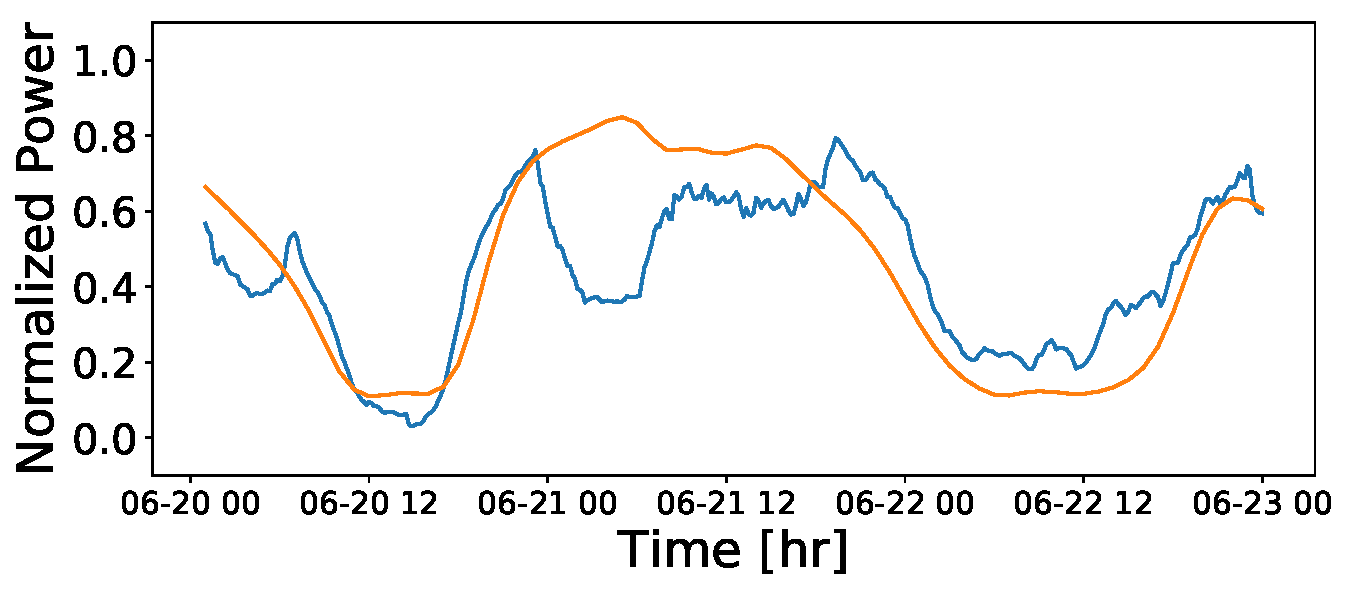
\includegraphics[width=70mm,scale=1]{plots/data_1529456400.pdf}
  % \caption{title}
\end{figure}
% Do you have more data? send it our way.
\end{frame}


\begin{frame}\frametitle{Data Skewness}
\begin{figure}
  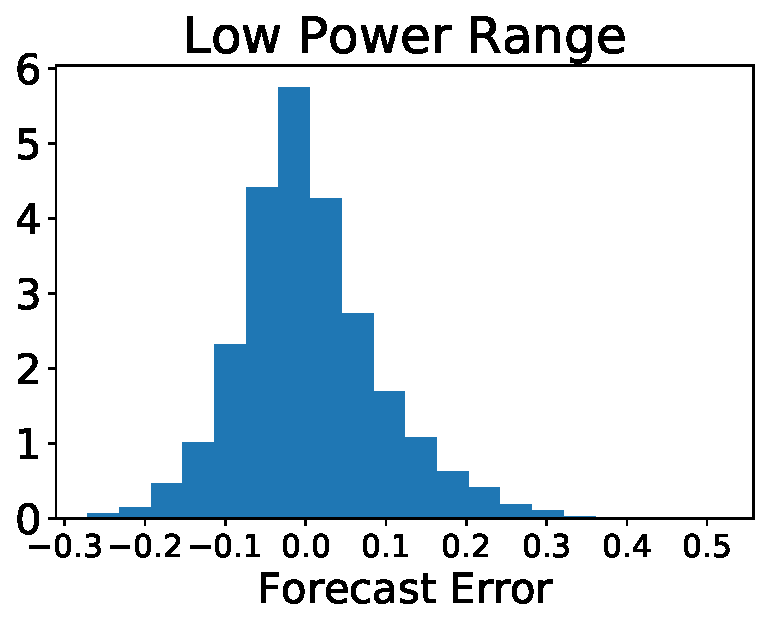
\includegraphics[width=47.5mm,scale=1]{plots/hist_low.pdf}
  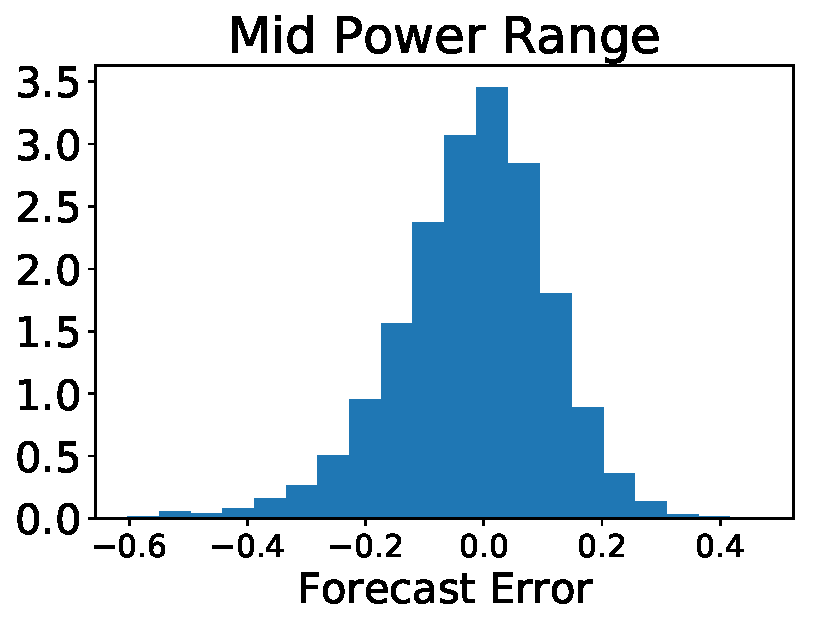
\includegraphics[width=50mm,scale=1]{plots/hist_mid.pdf}
  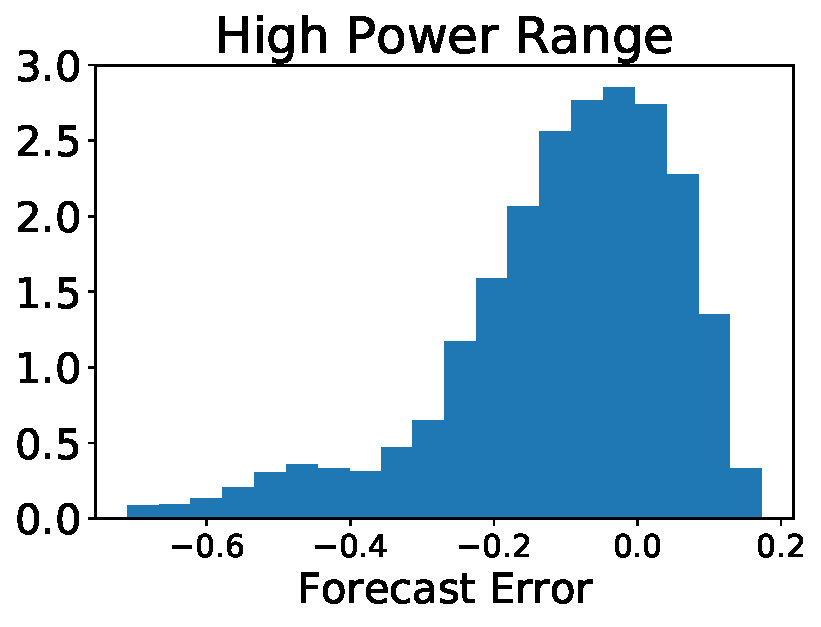
\includegraphics[width=50mm,scale=1]{plots/hist_high.pdf}
  \caption{We see that forecast errors exhibit skewness near the boundries (i.e. low and high power production regimes.)}
\end{figure}
\end{frame}

\begin{frame}\frametitle{Model}
Our goals are to
\begin{itemize}
  \item Generate a probabilistic forecast centered around a given deterministic forecast, i.e. unbiased with respect to the deterministic forecast.
  \item Capture the dynamics and correlation structure.
  \item Capture the skew nature of forecast errors.
  \item Be forecasting technology agnostic. Thus, compatible with future forecasting technology.
  \item Learn from historical power production data.
\end{itemize}
\end{frame}

\begin{frame}\frametitle{Model}
We propose to model wind power\textbf{ forecasts errors using parametric stochastic differential equations (SDEs)} whose solution defines a stochastic process. This resultant stochastic process describes the time evolution dynamics of wind power forecast errors.
\begin{equation}
\begin{split}
dX_t &= a(X_t; \bm{\theta}) dt + b (X_t; \bm{\theta} ) dW_t \quad t > 0 \\
X_0 & = X_0
\end{split}
\label{main}
\end{equation}

\begin{itemize}
\item $a(\cdot; \bm{\theta}):[0,1] \to \R $  a drift function.
\item $b (\cdot; \bm{\theta} ):[0,1] \to \R$  a  diffusion function.
\item $\bm{\theta}$: a vector of parameters.
\item $W_t$: Standard Wiener random process in $\R$.
\end{itemize}

Question: How do we choose an appropriate drift and diffusion functions?

\end{frame}


\begin{frame}\frametitle{Model}
Answer:
\begin{enumerate}
  \item We want the process to follow the wind forecast, thus we choose a drift term that is mean reverting and tracks the derivative of the deterministic forecast $p$, which is an input to our model.
  \begin{equation}
    a(X_t; \bm{\theta})=  \dot{p} \ dt - \theta_t(X_t - p_t)
  \end{equation}
where $\theta_t$ is a time-dependent paramter that controls the speed of reversion.
  \item We want a diffusion term that vanishes at the boundaries to prevent the process from escaping the region $[0,1]$.
  \begin{equation}
    b (\cdot; \bm{\theta} )= \sqrt{2 \theta_t \alpha x (1-x)}
  \end{equation}
  where $\alpha$ is a constant prameter that controls the path variability.

To further ensure that the process does not escape the region $[0,1]$, the mean reversion parameter has to be selected according to the following rule,
\begin{equation}
\theta_t = \max \left( \theta_0 \ , \ \frac{|\dot{p}_t|}{\min (p_t, 1-p_t)}  \right ) \label{theta_t}
\end{equation}
\end{enumerate}
\end{frame}

\begin{frame}\frametitle{Model}
Thus, our SDE becomes
\begin{equation}
\begin{split}
dX_t&= \dot{p}_t \ dt - \theta_t(X_t - p_t) \ dt + \sqrt{2 \theta_t \alpha x (1-x)}  \ dW_t \quad t > 0 \\
X_0&=x_0\\
% \theta_t &= \max \left( \theta_0 \ , \ \frac{|\dot{p}_t|}{\min (p_t, 1-p_t)}  \right )\\
\end{split}
\label{model:derivative_tracking_X}
\end{equation}
To avoid differentiation of the forecast $p_t$ and simplify, we apply a change of variables $$V_t = X_t - p_t$$ \\
The  model becomes,
\begin{equation}
\begin{split}
dV_t &=  - \theta_t V_t \  dt + \sqrt{2 \theta_t \alpha (V_t +p_t ) (1-V_t-p_t)} \  dW_t  \\ %\quad t > 0
V_0 & = v_0\\
% \theta_t &= \max \left( \theta_0 \ , \ \frac{|\dot{p}_t|}{\min (p_t, 1-p_t)}  \right )\\
\end{split}\label{VtSDE}
\end{equation}
Note that this model is Markovian.
\end{frame}

\begin{frame}\frametitle{Model}
Since $V_t$ defined by our SDE is Markovian, the likelihood function can be written as a product of transition densities.

\begin{equation}
\mathcal{L}(\bm{\theta};V) =\prod\limits_{j=1}^M \prod\limits_{i=1}^N \rho ( {V_{j,i+1}|V_{j,i}}, \bm{\theta})  \rho (V_{j,0})
\label{likelihood}
\end{equation}

The transition densities can be exactly obtained by solving the following parametric Fokker-Planck equation,

\begin{equation}
\begin{split}
\frac{ \partial f }{\partial t } & (y ,t | x , s, \theta_t, \alpha )= - \frac{\partial}{ \partial y} ( a( y;\dot{p}_t , p_t, \theta_t ) f( y ,t | x , s, \theta_t , \alpha ) ) \\
& + \frac{1}{2} \frac{\partial^2}{ \partial y^2} ( b(y;\theta_t, \alpha  )  f( y ,t | x , s, \theta_t , \alpha )  ) \quad  t < s\\
\end{split}
\end{equation}
This is a parametric PDE which is computationally prohibitive to solve and optimize for every transition.
\end{frame}


\begin{frame}\frametitle{Moment Matching}
Instead of solving for exact transition densities by the Fokker-Planck, we propose a \textbf{proxy transition denisty}. We match the moments of our SDE model with that of the proxy density. Using Ito, we arrive at the following iterative ODEs.

\begin{equation}
\begin{split}
\frac{d \E[ V^k_t]}{dt} = - k \theta_t \E [ V^k_t] + \frac{k(k-1)}{2} \E [ V^{k-2}_t  b(y;\theta_t, \alpha)]
\end{split}
\end{equation}
For the first two moments, we obtain
\begin{equation}
\begin{split}
\frac{d m_1 (t)}{dt} &= - m_1(t)\theta_t \\
\frac{d m_2 (t)}{dt} &=  -2 m_2(t)\theta(1+\alpha) + 2\alpha\theta m_1(t)(1-2p_t) + 2 \alpha\theta p_t (1-p_t)\\
\end{split}
\end{equation}

 A suitable candidate is a Beta transition density as it is compactly supported and can morph into symmetric and asymmetric shapes.

\end{frame}

\begin{frame}\frametitle{Algorithm}

Execute the following until an accuracy threshold is met:
\begin{enumerate}
\item initialize.
\item optimize the log-likelihood function.
\begin{enumerate}
\item For every evaluation of the log-liklihood function:
\begin{enumerate}
  \item Sample a batch of transitions and their associated forecast and parameters.
  \item Solve the ODE system for every transition.
  \item Match the resulting moments with the parameters of the chosen proxy distribution for every transition.
\end{enumerate}
\end{enumerate}
\item go to step 1 (i.e. re-initialize the optimization with the most recent result ).
\end{enumerate}

Notes:
\begin{itemize}
\item Choose your favorite deterministic optimization algorithm.
\item Choose your favorite integrator to solve the ODE system.
\end{itemize}
\end{frame}

\begin{frame}\frametitle{Inference Results}
Here we show the convergence path of the optimization in 2D, the likelihood in 3D and rate of the shrinking ellipses in one slide.
\end{frame}

\begin{frame}\frametitle{Simulation and Confidence Bands}
Here we show simulated future wind power production and another plot with confidence bands.
\end{frame}

\begin{frame}\frametitle{State-Independent model}
The model we have demostrated previously is state-dependent, that is the diffusion of the SDE depends on the state.
\begin{equation}
\begin{split}
dV_t &=  - \theta_t V_t \  dt + \sqrt{2 \theta_t \alpha (V_t +p_t ) (1-V_t-p_t)} \  dW_t  \\ %\quad t > 0
V_0 & = v_0\\
\end{split}\label{VtSDE}
\end{equation}

Why are we interested in a state-independent model? Because it's more tractable.\\
We apply a \textbf{Lamperti transform} to obtain the following state-independent system,

\begin{equation}
  \begin{split}
    dZ_t&= \frac{- \theta_t (1+ \sin(Z_t) - 2p_t) + \alpha \theta_t \sin (Z_t)   }{\cos (Z_t)} + \sqrt{2 \alpha \theta_t} dW_t \\
    Z_0&=z_0
  \end{split}
\end{equation}
where $Z_t = \arcsin \left( \frac{1}{2} \left( V_t+p_t \right) - 1 \right) $.
\end{frame}

\begin{frame}\frametitle{Data Skewness after Lamperti transformation}
As stated before, the state-independent SDE follows a Lamperti transformed process $Z_t$ give by $Z_t = \arcsin \left( \frac{1}{2} \left( V_t+p_t \right) - 1 \right) $.
\begin{figure}
  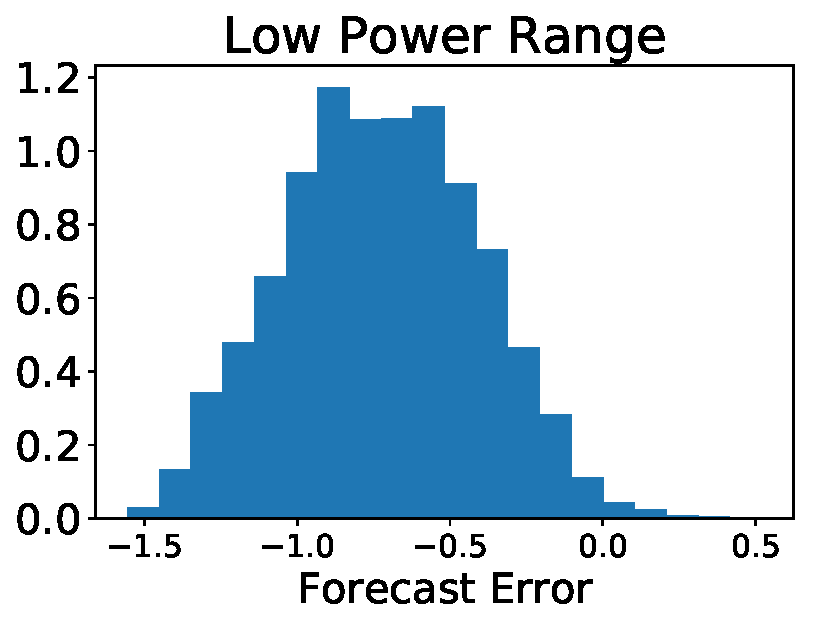
\includegraphics[width=50mm,scale=1]{plots/hist_low_lamperti.pdf}
  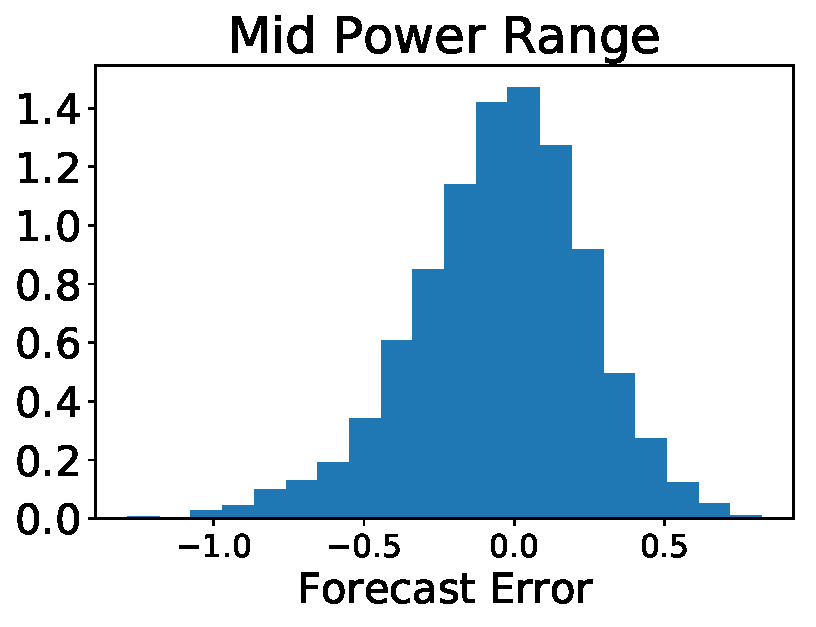
\includegraphics[width=50mm,scale=1]{plots/hist_mid_lamperti.pdf}
  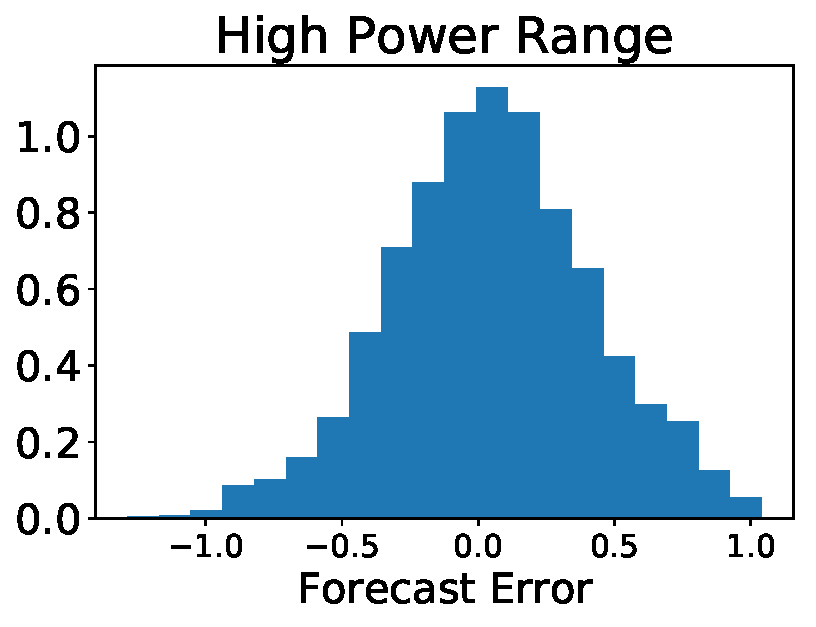
\includegraphics[width=50mm,scale=1]{plots/hist_high_lamperti.pdf}
  \caption{We observe that most of the skewness has been removed after the lamperti transformation. This motivates us to use a Gaussian transition density as a proxy denisty.}
\end{figure}
\end{frame}

\begin{frame}\frametitle{State-Independent model}
Similarly, we try to obtain a system of ODEs to determine the centered moments of the Lamperti transformed process $V_t$. Due to the non-linearity in the drift, we can only approximate the centered moments by the following ODEs,
\begin{equation}
\begin{split}
\frac{d m_1 (t)}{dt} &= - m_1(t)\theta_t (1-\alpha) - \theta (1-2 p_t) \\
\frac{d v(t)}{dt} &=  2 v(t) \theta_t (2p_t - 1 ) \tan(x) \sec(x) + \theta_t (\alpha - 1) \sec^2(x)  + 2 \theta_t \alpha\\
\end{split}
\end{equation}
These are not exact moment ODEs, however they are good enough for small time intervals.
\end{frame}

\begin{frame}\frametitle{Inference Results}
Here we show the convergence path of the optimization in 2D, the likelihood in 3D and rate of the shrinking ellipses in one slide.
\end{frame}

\begin{frame}\frametitle{Simulation and Confidence Bands}
Here we show simulated future wind power production and another plot with confidence bands.
\end{frame}

\begin{frame}\frametitle{Model comparison}
\begin{table}[]
\centering
\begin{tabular}{|c|c|c|c|}
\hline
Model   &  parameters $(\theta_0, \alpha)$   & AIC & BIC \\ \hline
state-dependent &   (,)  &     &      \\ \hline
state-independent &   (,)  &     &       \\ \hline
\end{tabular}
\caption{We compare the two models based on information criterion here.... }
\label{tab:model_comparison}
\end{table}
\end{frame}

\begin{frame}\frametitle{Concluding remarks}
We were able to:
\begin{itemize}
  \item simulate future wind power production based on real data.
  \item have an analytical description of the uncertainty of wind power forecasts in the form of an SDE.
  \item develop a forecasting technology agnostic method.
  \item capture skewness of the error process and its correlation structure.
\end{itemize}
\end{frame}


\begin{frame}\frametitle{References}
\begin{itemize}
  \item source
  \item source
  \item source
\end{itemize}
\end{frame}


\end{document}
